\documentclass{article}
\usepackage{tikz}
\usetikzlibrary{arrows.meta,positioning,calc,shapes.geometric}
\pagestyle{empty}
\begin{document}
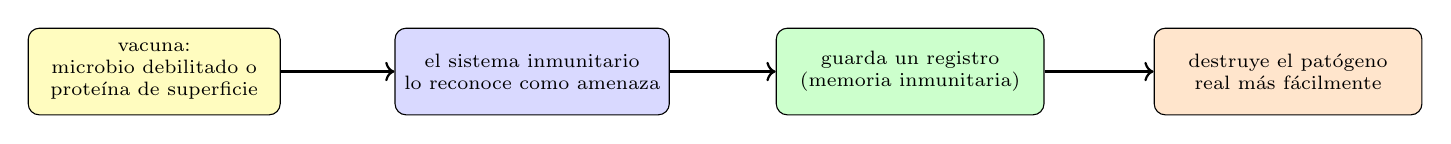
\begin{tikzpicture}
\tikzset{every node/.append style={align=center}}

\node[draw, rounded corners, fill=yellow!25, minimum width=3.2cm, minimum height=1.1cm, align=center, font=\scriptsize] (a) at (0,0) {vacuna:\\ microbio debilitado o\\ proteína de superficie};
\node[draw, rounded corners, fill=blue!15, minimum width=3.4cm, minimum height=1.1cm, align=center, font=\scriptsize] (b) at (4.8,0) {el sistema inmunitario\\ lo reconoce como amenaza};
\node[draw, rounded corners, fill=green!20, minimum width=3.4cm, minimum height=1.1cm, align=center, font=\scriptsize] (c) at (9.6,0) {guarda un registro\\ (memoria inmunitaria)};
\node[draw, rounded corners, fill=orange!20, minimum width=3.4cm, minimum height=1.1cm, align=center, font=\scriptsize] (d) at (14.4,0) {destruye el patógeno\\ real más fácilmente};
\draw[->, thick] (a) -- (b); \draw[->, thick] (b) -- (c); \draw[->, thick] (c) -- (d);

\end{tikzpicture}
\end{document}
